
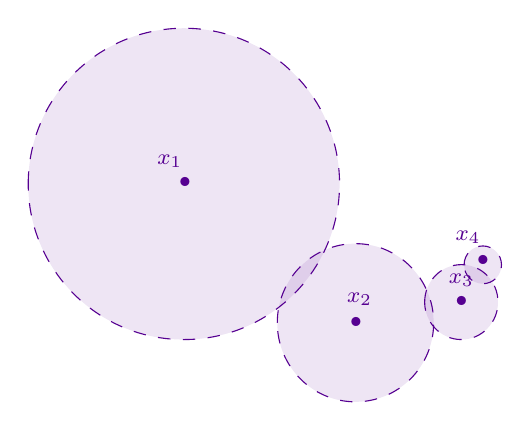
\begin{tikzpicture}[x=0.75pt,y=0.75pt,yscale=-1,xscale=1]
	%uncomment if require: \path (0,300); %set diagram left start at 0, and has height of 300

	%Shape: Ellipse [id:dp7658406221599783] 
	\draw  [color={rgb, 255:red, 86; green, 0; blue, 145 }  ,draw opacity=1 ][fill={rgb, 255:red, 86; green, 0; blue, 145 }  ,fill opacity=0.1 ][dash pattern={on 4.5pt off 4.5pt}] (0,75) .. controls (0,33.58) and (33.58,0) .. (75,0) .. controls (116.42,0) and (150,33.58) .. (150,75) .. controls (150,116.42) and (116.42,150) .. (75,150) .. controls (33.58,150) and (0,116.42) .. (0,75) -- cycle ;

	%Shape: Ellipse [id:dp6629907428161504] 
	\draw  [color={rgb, 255:red, 86; green, 0; blue, 145 }  ,draw opacity=1 ][fill={rgb, 255:red, 86; green, 0; blue, 145 }  ,fill opacity=0.1 ][dash pattern={on 4.5pt off 4.5pt}] (120,141.9) .. controls (120,120.85) and (136.86,103.79) .. (157.67,103.79) .. controls (178.47,103.79) and (195.33,120.85) .. (195.33,141.9) .. controls (195.33,162.94) and (178.47,180) .. (157.67,180) .. controls (136.86,180) and (120,162.94) .. (120,141.9) -- cycle ;
	%Shape: Ellipse [id:dp09734770391428005] 
	\draw  [color={rgb, 255:red, 86; green, 0; blue, 145 }  ,draw opacity=1 ][fill={rgb, 255:red, 86; green, 0; blue, 145 }  ,fill opacity=0.1 ][dash pattern={on 4.5pt off 4.5pt}] (191,131.95) .. controls (191,121.98) and (198.91,113.9) .. (208.67,113.9) .. controls (218.42,113.9) and (226.33,121.98) .. (226.33,131.95) .. controls (226.33,141.92) and (218.42,150) .. (208.67,150) .. controls (198.91,150) and (191,141.92) .. (191,131.95) -- cycle ;
	%Shape: Ellipse [id:dp1342431229797264] 
	\draw  [color={rgb, 255:red, 86; green, 0; blue, 145 }  ,draw opacity=1 ][fill={rgb, 255:red, 86; green, 0; blue, 145 }  ,fill opacity=0.1 ][dash pattern={on 4.5pt off 4.5pt}] (210,114) .. controls (210,108.97) and (214.03,104.9) .. (219.01,104.9) .. controls (223.99,104.9) and (228.02,108.97) .. (228.02,114) .. controls (228.02,119.03) and (223.99,123.1) .. (219.01,123.1) .. controls (214.03,123.1) and (210,119.03) .. (210,114) -- cycle ;

	% Text Node
	\draw (61,60) node [anchor=north west][inner sep=0.75pt]  [font=\footnotesize,color={rgb, 255:red, 86; green, 0; blue, 145 }  ,opacity=1 ]  {$x_{1}$};
	% Text Node
	\draw (75.5,74.5) node  [font=\footnotesize,color={rgb, 255:red, 86; green, 0; blue, 145 }  ,opacity=1 ]  {$\bullet $};
	% Text Node
	\draw (201.4,117) node [anchor=north west][inner sep=0.75pt]  [font=\footnotesize,color={rgb, 255:red, 86; green, 0; blue, 145 }  ,opacity=1 ]  {$x_{3}$};
	% Text Node
	\draw (208.78,131.83) node  [font=\footnotesize,color={rgb, 255:red, 86; green, 0; blue, 145 }  ,opacity=1 ]  {$\bullet $};
	% Text Node
	\draw (152.4,126.08) node [anchor=north west][inner sep=0.75pt]  [font=\footnotesize,color={rgb, 255:red, 86; green, 0; blue, 145 }  ,opacity=1 ]  {$x_{2}$};
	% Text Node
	\draw (157.92,141.64) node  [font=\footnotesize,color={rgb, 255:red, 86; green, 0; blue, 145 }  ,opacity=1 ]  {$\bullet $};
	% Text Node
	\draw (204.61,96.47) node [anchor=north west][inner sep=0.75pt]  [font=\footnotesize,color={rgb, 255:red, 86; green, 0; blue, 145 }  ,opacity=1 ]  {$x_{4}$};
	% Text Node
	\draw (219.07,111.94) node  [font=\footnotesize,color={rgb, 255:red, 86; green, 0; blue, 145 }  ,opacity=1 ]  {$\bullet $};
	% Text Node
	\draw (219,95.5) node  [font=\footnotesize,color={rgb, 255:red, 86; green, 0; blue, 145 }  ,opacity=1 ,rotate=-283.93]  {$\dotsc $};


\end{tikzpicture}
